Obwohl die Nutzung von OSS Folgen für das gesamte DevOps-Team hat, wird die Entscheidung über die Nutzung von der Rolle des Entwicklers getroffen, wodurch die Prozessanpassungen vorrangig im Bereich der Entwicklung vorgenommen werden müssen. 

Wie auch bei dem Prozessmodel des IST-Zustandes wurde der Gesamtprozess, zum besseren Verständnis in drei Teile aufgeteilt, die wiederrum einzeln (Abbildung 14 - 16) erläutert werden. 

Auch wurde ausschließlich die Rolle des Entwicklerteams, mit einem entsprechenden Start und Endpunkt modelliert und die Rolle des Product Owners nicht weiter behandelt, da für die Verwendung von OSS in den DevOps-Produktentwicklungsprozess keine direkten Auswirkungen für den Product Owner bestehen.

\begin{figure}[p]
    \centering
    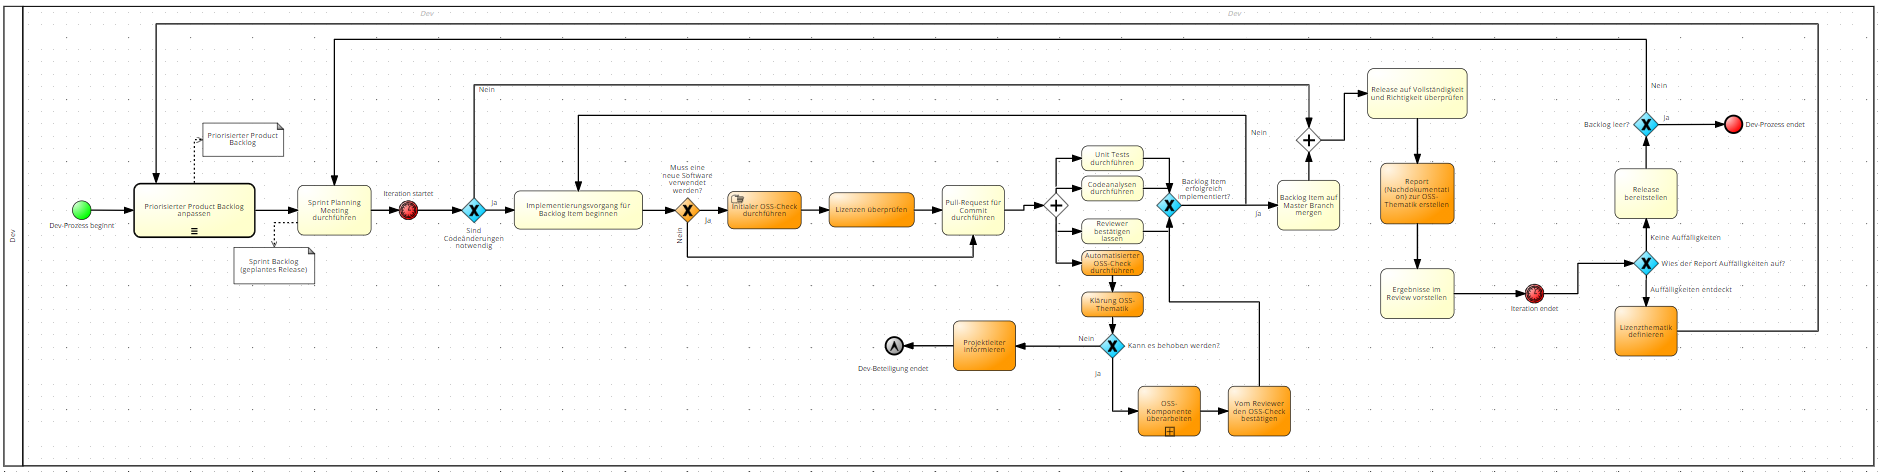
\includegraphics[angle=90, scale=0.5]{Bilder/SOLL-Prozess.png}
    \caption{Einbindung von OSS in den Softwareentwicklungsprozess basierend auf dem internen msg-Projekt}
\end{figure}

Da zu dem Zeitpunkt der Nutzung von OSS die Projektstruktur bereits besteht und das Product Backlog ebenfalls erstellt wurde, bildet den Anfang des Softwareentwicklungsprozesses nun die Anpassung des priorisierten Product Backlogs.

\begin{figure}[h]
    \centering
    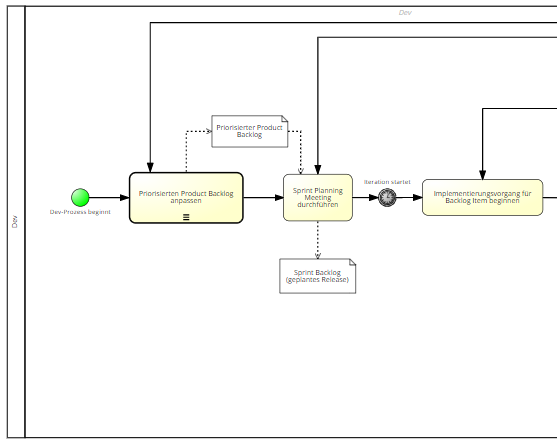
\includegraphics[scale=0.5]{Bilder/SOLL-Prozess_first Part.png}
    \caption{Erster Teil des Softwareentwicklungsprozess im SOLL-Zustand basierend auf dem HAF-Projekt}
\end{figure}

Nachdem das Sprint Planning Meeting durchgeführt worden ist, kann die Iteration basierend auf den Anforderungen aus dem Sprint Backlog, gestartet werden, wodurch der Implmentierungsvorgang für die jeweiligen Sprint Backlog Items beginnen kann.

In diesem Rahmen sind Codeänderungen notwendig, die sich auf vorhandenen Code oder eine Neuimplementierung beziehen können.

Ab diesem Zeitpunkt setzt die Nutzung von OSS die Prozessänderungen in Gang.

\begin{figure}[h]
    \centering
    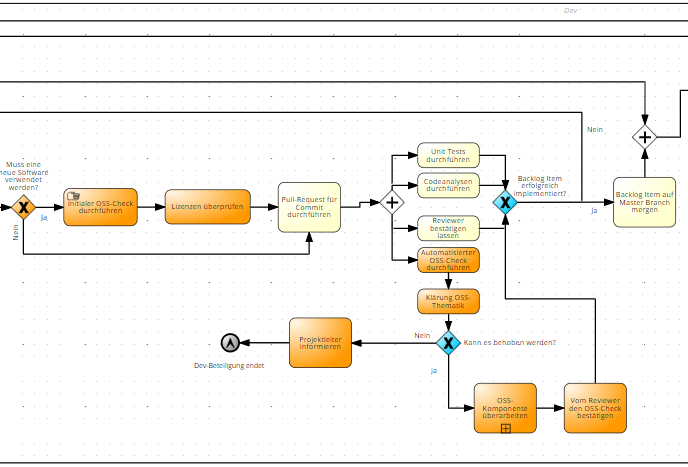
\includegraphics[scale=0.5]{Bilder/SOLL-Prozess_second Part.png}
    \caption{Zweiter Teil des Softwareentwicklungsprozess im SOLL-Zustand basierend auf dem internene msg-Projekt}
\end{figure}

Um präventiv maßgebliche Konsequenzen durch die Nutzung von OSS zu vermeiden, sollten sich die betreffenden Entwickler die Frage stellen, ob tatsächliche eine neue Software oder Softwarekomponete in das Projekt eingebunden werden muss. 

Falls dies der Fall ist, muss zunächst ein initaler OSS-Check durchgeführt werden. 

Dieser dient dazu, das Lizenzmodell der verwendeten OSS-Komponete manuell zu überprüfen und diese mit den 'ungefährlichen' Lizenzmodellen zu vergleichen. 

Dies hat zum Vorteil, dass der Entwickler bereits vor einer langen Implementierung eine Aussage darüber treffen kann, ob sich aus Sicht der Lizenzmodelle eine Verwendung eignet oder ob ein Lizenzmodell vorliegt, welches zumindest ein beschränktes Copyleft aufweist.

Die entsprechende manuelle Checkliste wird im Kapitel 3.3 ausführlich behandelt. 

Sollte die verwendete OSS-Komponete ein derartiges Lizenzmodell aufweisen, hat der Entwickler ausreichend Zeit, nach eine 'ungefährlichen' Alternative zu suchen.  

Wird die OSS-Kompoente letztlich verwendet, wird ein Pull-Request für ein Commit durchgeführt. 

An diesem Punkt befindet sich der Entwickler ebenfalls, wenn keine neue OSS genutzt wird. 

Anschließend hierzu werden wie im regelmäßigen Prozess, Unit-Tests und Codeanalysen durchgeführt.

Gleichzeitig zu diesen Schritten muss erneut eine neue Anpassung des Prozesses im Hinblick auf die Verwendung von OSS als ein automatisierten OSS-Check durchgeführt werden.

Während bei einer Verwendung von neuer OSS die Lizenzmodelle zeitnah überprüft werden können, kann es Fälle geben, in denen Versionen einer bereits implementierten OSS-Komponete geändert werden und daraus eine Verschiebung der betreffenden Lizenzmodelle stattfinden kann. 

Dies kann zur Folge haben, dass OSS-Komponeten ein starkes Copyleft aufweisen, obwohl diese mit einem schwachen oder keinen Copyleft anfänglich implementiert worden sind. 

Ferner würde diese Situation bei einer gängigen Entwicklung nicht auffallen und bietet daher ein großes Risiko für das Unternehmen als auch für das entsprechende Entwicklerteam. 

Durch einen automatisierten OSS-Check können die Lizenzmodelle der verwendeten OSS-Komponeten anhand ihrer Versionen dargestellt werden. 

Damit erhalten alle Entwickler einen genauen Überblick über die verwendeten OSS-Komponeten und deren akutellen Lizenzstatus. 

Zu beachten ist dabei, dass der automatisierte OSS-Check nach jedem Commit ausgeführt werden muss, damit die Entwickler genug Zeit haben, nach einer Lösung für eine mögliche Lizenzproblematik zu suchen.

Durch die zeitnahe Übermittlung der notwendigen Informationen wird die Transparenz zwischen den DevOps-Mitgliedern sichergestellt. 

Die Automatisierung des OSS-Checks entspricht sowohl der Kultur als auch den Methoden nach den DevOps-Prinzipien.

Sollte die Überprüfung mittels des automatisierten OSS-Checks kein schwieriges Copyleft finden, wird das Commit, wie im gängigen Softwareentwicklungsprozess, zunächst vom Reviewer bestätigt und kann dann als Backlog Item erfolgreich implementiert und auf das Master Branch gemergt werden. 

Falls dies nicht der Fall ist und eine OSS-Komponete ein nicht gewünschtes Lizenzmodell aufweisen, muss die OSS-Thematik zunächst geklärt werden.

Sollte die entstandene Problematik nicht behoben werden, so muss der Projektleiter informiert werden und die Dev-Beteiligung endet zunächst an dieser Stelle. 

Kann das Problem im Hinblick auf die OSS-Komponete behoben werden, muss diese zunächst überarbeitet werden. 

Dies reicht von einem Rückgang auf eine alte Version, wobei an dieser Stelle die gesamte Funktionalität gewährleistet werden muss, bis zur Verwerfung der entsprechenden Kompoente durch den Entwickler. 

Dieser Aufgabenbereich kann mehrere Unteraufgaben aufweisen und die Lösung ist demnach spezifisch auf die Komponete und deren Entwicklung ausgelegt. 

Nach der Überarbeitung erfolgt eine Bestätigung durch einen Reviewer, zum Ziel, die Kompoente erfolgreich auf den Master Branch zu mergen. 
\dwi{hier fehlen wieder die referenzen auf die abbildungen! darüber hinaus gilt hier umso mehr (du hast ja neues wissen/neue prozesschritte), dass die elemente der grafik klar und einfach dem text zuzuordnen sind. hier wäre die gleiche art auflistung mit gleicher nummerierung in der grafik sehr geschickt.}

\begin{figure}[h]
    \centering
    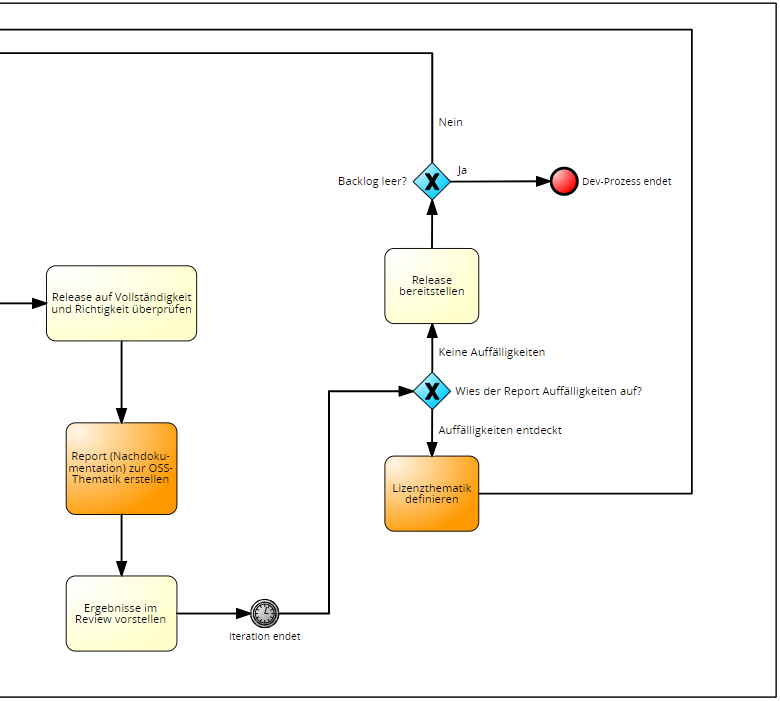
\includegraphics[scale=0.5]{Bilder/SOLL-Prozess_third Part.png}
    \caption{Dritter Teil des Softwareentwicklungsprozess im SOLL-Zustand basierend auf dem internen msg-Projekt}
\end{figure}

Sobald das Release auf seine Vollständigkeit und Richtigkeit überprüft worden ist, wird zur erneuten Kontrolle der Lizenzmodelle ein Report erstellt. 

Dieser dient als eine Nachdokumentation, einerseits falls sich unbeabsichtigt Änderungen ergeben haben, die bisher nicht gesehen wurden und andererseits zur Vorlage für den Stakeholder, um den Status der verwendeten OSS-Komponeten transparent zu präsentieren. 

Die Iteration endet mit der Vorstellung der Ergebnisse im Review. 

Basierend auf der Nachdokumentation muss anschließend analysiert werden, ob Auffälligkeiten innerhalb der Lizenzthematik festgestellt wurden.  

Ergeben sich tatsächlich Auffälligkeiten, müssen diese zunächst definiert und innerhalb des Product Backlog übermittelt werden. 

Müssen keine Veränderungen vorgenommen werden, wird das Release bereitgestellt. 

Genau wie bei dem gängigen Softwareentwicklungsprozess im IST-Zustand, endet dieser Prozess ebenfalls mit einem leeren Product Backlog.  

















